\documentclass[11pt,onecolumn,letterpaper]{article}
\usepackage[spanish]{babel}
\usepackage[utf8]{inputenc}
\usepackage[T1]{fontenc}
\usepackage[a4paper,top=2.2cm,bottom=2.3cm,left=2.2cm,right=2.2cm]{geometry}

\usepackage{amsmath,amssymb,mathtools}
\usepackage{graphicx}
\usepackage{booktabs}
\usepackage{array}
\usepackage{multirow}
\usepackage{xcolor}
\usepackage{float}
\usepackage[shortlabels]{enumitem}
\usepackage{listings}
\usepackage{lmodern}
\usepackage{caption}
\usepackage{subcaption}
\usepackage{tikz}
\usetikzlibrary{positioning,arrows.meta,shapes.geometric,calc,decorations.pathreplacing,decorations.markings,fit}
\usepackage{pgfplots}
\pgfplotsset{compat=1.18}
\usepackage[colorlinks=true, linkcolor=blue, citecolor=blue, urlcolor=cyan, filecolor=magenta]{hyperref}

% ----------------------------------------------------------------------------
% Estilo de código (Python), usado para referenciar fragmentos reales del repo
% ----------------------------------------------------------------------------
\definecolor{codegreen}{rgb}{0,0.5,0}
\definecolor{codegray}{rgb}{0.5,0.5,0.5}
\definecolor{codepurple}{rgb}{0.58,0,0.82}
\definecolor{backcolour}{rgb}{0.96,0.96,0.94}

\lstdefinestyle{mystyle}{
    backgroundcolor=\color{backcolour},
    commentstyle=\color{codegreen},
    keywordstyle=\color{magenta},
    numberstyle=\tiny\color{codegray},
    stringstyle=\color{codepurple},
    basicstyle=\ttfamily\footnotesize,
    breakatwhitespace=false,
    breaklines=true,
    captionpos=b,
    keepspaces=true,
    numbers=left,
    numbersep=6pt,
    showspaces=false,
    showstringspaces=false,
    showtabs=false,
    tabsize=2,
    language=Python,
    frame=single,
    rulecolor=\color{black!20},
}
\lstset{style=mystyle}

\newcommand{\code}[1]{\texttt{#1}}

% ----------------------------------------------------------------------------
% Encabezado académico compacto (adaptado de la plantilla de Tarea 1; sin
% logos porque no están disponibles en este repo)
% ----------------------------------------------------------------------------
\newcommand{\tituloTrabajo}{Tarea 2}
\newcommand{\materia}{Inteligencia Artificial 2027-I}
\newcommand{\subtituloTrabajo}{CSP, Metaheur\'isticas y B\'usqueda con Adversarios}
\newcommand{\alumno}{Diego Antonio Villalba Gonz\'alez}

\newcommand{\makecourseheader}{%
    \begingroup
    \setlength{\parindent}{0pt}%
    \noindent
    {\sffamily\color{black!65}\normalsize UNIVERSIDAD NACIONAL AUT\'ONOMA DE M\'EXICO \\
    \footnotesize\bfseries Posgrado en Ciencias e Ingenier\'ia de la Computaci\'on}\par
    \vspace{0.22cm}
    \sffamily
    {\LARGE\bfseries\color{black!90}\tituloTrabajo}\par
    \vspace{0.06cm}
    {\large\color{black!70}\subtituloTrabajo}\par
    \vspace{0.22cm}
    {\small
    \textbf{Materia:} \materia\\[-0.02cm]
    \textbf{Alumno:} \alumno\\[-0.02cm]
    \textbf{Fecha:} \today
    }
    \vspace{0.3cm}
    {\color{black!25}\hrule height 0.6pt}
    \vspace{0.5cm}
    \endgroup
}

% ----------------------------------------------------------------------------
% Macro para dibujar tableros de gato 3x3 compactos (usado en Ejercicio 3)
% ----------------------------------------------------------------------------
\newcommand{\tttboard}[9]{%
  \begin{tikzpicture}[baseline=-0.5ex, scale=1]
    \draw[black!70] (0,0) rectangle (1.05,1.05);
    \draw[black!70] (0.35,0) -- (0.35,1.05);
    \draw[black!70] (0.70,0) -- (0.70,1.05);
    \draw[black!70] (0,0.35) -- (1.05,0.35);
    \draw[black!70] (0,0.70) -- (1.05,0.70);
    \node[font=\tiny] at (0.175,0.875) {#1};
    \node[font=\tiny] at (0.525,0.875) {#2};
    \node[font=\tiny] at (0.875,0.875) {#3};
    \node[font=\tiny] at (0.175,0.525) {#4};
    \node[font=\tiny] at (0.525,0.525) {#5};
    \node[font=\tiny] at (0.875,0.525) {#6};
    \node[font=\tiny] at (0.175,0.175) {#7};
    \node[font=\tiny] at (0.525,0.175) {#8};
    \node[font=\tiny] at (0.875,0.175) {#9};
  \end{tikzpicture}%
}

\title{\tituloTrabajo}
\date{}

\begin{document}
\sloppy
\makecourseheader

\tableofcontents
\vspace{0.4cm}

% =============================================================================
\section{Partes resueltas}
% =============================================================================

Como lo pide el enunciado, esta tabla indica expl\'icitamente qu\'e partes de la tarea se
resolvieron y d\'onde se encuentra cada una en este reporte y en el c\'odigo (repositorio
completo, con instrucciones de reproducci\'on, en \code{README.md}).

\begin{center}
\small
\begin{tabular}{@{}p{7.7cm}p{2.1cm}p{5.6cm}@{}}
\toprule
\textbf{Parte del enunciado} & \textbf{Estado} & \textbf{Secci\'on / c\'odigo} \\
\midrule
Cr\'itica: T\"onshoff et al. (2023) & Completo & \S\ref{sec:readings-tonshoff} \\
Cr\'itica: Doerr et al. (2024) & Completo & \S\ref{sec:readings-doerr} \\
Backtracking + rev.\ hacia adelante + AC-3 + ordenamiento & Completo & \S\ref{sec:impl-csp}, \code{src/csp/} \\
Metaheur\'istica (recocido simulado) & Completo & \S\ref{sec:impl-sa}, \code{src/metaheuristics/} \\
Minimax & Completo & \S\ref{sec:impl-minimax}, \code{src/adversarial/minimax.py} \\
N-reinas $N=8$ y $N=100$ (backtracking + metaheur\'istica) & Completo & \S\ref{sec:app-nqueens} \\
Todas las soluciones de N-reinas $N=100$ & Completo (acotado, no exhaustivo; se justifica por qu\'e) & \S\ref{sec:app-enum} \\
Coloreado de grafos, 50 nodos (backtracking + metaheur\'istica) & Completo & \S\ref{sec:app-coloring} \\
Coloreado de grafos, 1000 nodos (backtracking + metaheur\'istica) & Parcial (acotado: $49\le\chi\le302$; se justifica por qu\'e) & \S\ref{sec:app-coloring} \\
Coloreado vs.\ OR-Tools, 50 nodos & Completo & \S\ref{sec:app-ortools} \\
Coloreado vs.\ OR-Tools, 1000 nodos & Parcial (cota superior v\'ia OR-Tools, sin certificado de optimalidad) & \S\ref{sec:app-ortools} \\
Gato (gym-tic-tac-toe) con minimax & Completo & \S\ref{sec:app-tictactoe} \\
Ejercicio 1 (caballos como CSP) & Completo & \S\ref{sec:ex1} \\
Ejercicio 2 (Sudoku con b\'usqueda local) & Completo & \S\ref{sec:ex2} \\
Ejercicio 3 (\'arbol de juego del gato) & Completo & \S\ref{sec:ex3} \\
Ejercicio 4 (correctud de poda alfa-beta) & Completo & \S\ref{sec:ex4} \\
C\'odigo funcional + instrucciones de reproducci\'on & Completo & \S\ref{sec:repro}, \code{README.md} (13 pruebas unitarias, todas pasan) \\
\bottomrule
\end{tabular}
\end{center}

\noindent\textbf{Nota sobre alfa-beta}: el rubro de implementaci\'on (45 pts) solo pide
Minimax; por eso \code{src/adversarial/alpha\_beta.py} se deja intencionalmente vac\'io
-- alfa-beta se resuelve de forma te\'orica en el Ejercicio 4 (\S\ref{sec:ex4}), y
computacionalmente no hac\'ia falta: el \'arbol completo del gato es lo bastante peque\~no
para que minimax puro lo resuelva instant\'aneamente (ver \S\ref{sec:app-tictactoe}).

% =============================================================================
\section{Cr\'itica de lecturas}
% =============================================================================

\subsection{T\"onshoff, Kisin, Lindner y Grohe (2023) --- \emph{One Model, Any CSP}~\cite{tonshoff2023onemodel}}
\label{sec:readings-tonshoff}

El problema que atacan es que los solucionadores de CSP basados en b\'usqueda local
(recocido simulado, min-conflicts, WalkSAT, \dots) suelen requerir una heur\'istica y una
funci\'on de vecindad dise\~nadas a mano \emph{para cada clase de problema}: una para
coloreado de grafos, otra para SAT, otra para programaci\'on de horarios, etc. Los autores
proponen \textsc{Any-CSP}: una \'unica red neuronal de grafos (GNN) recurrente que opera
directamente sobre el grafo de restricciones de \emph{cualquier} CSP (variables y
restricciones como nodos, sin importar su aridad o tipo) y, mediante pasos iterativos de
paso de mensajes, refina una distribuci\'on de probabilidad sobre valores para cada
variable hasta converger a una asignaci\'on. El modelo se entrena una sola vez sobre una
mezcla de clases de problemas (coloreado de grafos, MAX-2SAT, CSPs aleatorios, entre
otros) y luego se aplica sin reentrenar a instancias nuevas, incluso de clases o tama\~nos
no vistos durante el entrenamiento.

Los resultados que reportan son fuertes: en las instancias evaluadas, \textsc{Any-CSP}
iguala o supera tanto a heur\'isticas de b\'usqueda local especializadas como a trabajos
previos de GNNs entrenados espec\'ificamente por clase de problema, y generaliza
razonablemente bien a tama\~nos mayores a los vistos en entrenamiento. La limitaci\'on que
me parece m\'as relevante es que, como toda b\'usqueda local heur\'istica, \textsc{Any-CSP}
no ofrece garant\'ia de completitud: no puede certificar que un CSP es insatisfacible (a
diferencia de AC-3 + backtracking, que si vac\'ia un dominio, prueba insatisfacibilidad de
forma exacta), y su ``horizonte de razonamiento'' est\'a acotado por la profundidad de
paso de mensajes de la red, de manera an\'aloga a c\'omo forward checking o AC-3 solo
propagan consistencia de arco de alcance limitado en lugar de consistencia global.

La conexi\'on con lo implementado aqu\'i es directa: nuestro propio pipeline de
backtracking (\S\ref{sec:impl-csp}) usa heur\'isticas \emph{dise\~nadas a mano}
(MRV/LCV) para decidir qu\'e variable y valor probar primero, exactamente el tipo de
decisi\'on que \textsc{Any-CSP} aprende de datos en lugar de codificar. Esto es
particularmente relevante para el resultado menos satisfactorio de este trabajo: el
coloreado del grafo de 1000 nodos (\S\ref{sec:app-coloring}), donde ni backtracking con
MRV/LCV ni recocido simulado logran cerrar el n\'umero crom\'atico en un tiempo razonable.
Un modelo como \textsc{Any-CSP}, entrenado sobre instancias de coloreado similares,
podr\'ia potencialmente producir una coloraci\'on inicial de mejor calidad much\'isimo m\'as
r\'apido que un barrido de $k$ con backtracking exacto -- a costa, claro, de perder la
garant\'ia de optimalidad/completitud que s\'i tienen backtracking y OR-Tools.

\subsection{Doerr, Echarghaoui, Jamal y Krejca (2024) --- \emph{Runtime Analysis of the $(\mu+1)$ GA}~\cite{doerr2024runtime}}
\label{sec:readings-doerr}

Este trabajo pertenece al \'area de an\'alisis de tiempo de ejecuci\'on de algoritmos
evolutivos: en lugar de medir tiempos emp\'iricamente sobre benchmarks (como hacemos
nosotros en \S\ref{sec:app-nqueens}--\ref{sec:app-coloring}), los autores demuestran cotas
\emph{formales} sobre el n\'umero esperado de evaluaciones que necesita el algoritmo
gen\'etico $(\mu+1)$ para optimizar funciones de prueba est\'andar del \'area. La variante
que analizan mantiene una poblaci\'on de $\mu$ individuos y aplica un mecanismo expl\'icito
que descarta duplicados/individuos demasiado similares, generando lo que llaman ``fuerte
deriva hacia poblaciones diversas''. Su resultado principal es que esta presi\'on hacia la
diversidad produce mejoras \emph{demostrables} (no solo observadas emp\'iricamente) en el
tiempo esperado de optimizaci\'on frente tanto al algoritmo $(1+1)$ EA (que optimiza un
solo individuo a la vez, sin poblaci\'on) como frente a variantes de $(\mu+1)$ sin ese
mecanismo de diversidad.

La idea central -- diversidad poblacional como mecanismo para explorar varias cuencas de
atracci\'on simult\'aneamente, en lugar de una b\'usqueda de trayectoria \'unica que solo
puede escapar de un m\'inimo local reiniciando o calentando -- se conecta directamente con
nuestro recocido simulado (\S\ref{sec:impl-sa}), que es exactamente una b\'usqueda de
\emph{una sola trayectoria}: el an\'alogo m\'as cercano al $(1+1)$ EA que el propio paper usa
como punto de comparaci\'on m\'as d\'ebil. En la Secci\'on~7 (exploratoria, no pedida por el
enunciado) de \code{notebooks/results.ipynb} se observa evidencia consistente con esto:
de 9 corridas de recocido simulado sobre N-reinas $N=100$, la \'unica que no converge es
justamente la del scheduler \emph{sinusoidal} con semilla 1, que qued\'o con 1 conflicto
tras 100{,}000 iteraciones -- una \'unica trayectoria oscilando cerca de un \'optimo sin
lograr alcanzarlo. El resultado de Doerr et al.\ sugiere que mantener varias asignaciones
candidatas en paralelo, forz\'andolas a mantenerse diversas (en el esp\'iritu de un
algoritmo gen\'etico, la tercera opci\'on de metaheur\'istica que permit\'ia el enunciado),
podr\'ia ser una v\'ia con respaldo te\'orico -- no solo intuici\'on -- para atacar
justamente los casos donde nuestra \'unica trayectoria de recocido simulado se estanca,
como el coloreado del grafo de 1000 nodos cerca de su umbral real. La limitaci\'on que hay
que reconocer es que las cotas del paper son para funciones de prueba sint\'eticas del
\'area de teor\'ia de tiempos de ejecuci\'on, no para CSPs combinatorios como coloreado de
grafos o N-reinas; que el argumento se transfiera a nuestros problemas es una conjetura
razonable, no algo que el paper demuestre.

% =============================================================================
\section{Implementaci\'on}
% =============================================================================

Todo el c\'odigo referenciado en esta secci\'on vive en \code{src/} y se ejecuta,
extremo a extremo, desde los scripts de \code{experiments/} (ver \S\ref{sec:repro} y
\code{README.md} para los comandos exactos). El dise\~no separa, en todos los casos, el
motor gen\'erico de b\'usqueda (que no sabe nada de reinas, grafos o gatos) de la
definici\'on de cada problema concreto -- la misma separaci\'on que usa AIMA entre
``el algoritmo'' y ``el problema''.

\subsection{CSP gen\'erico: backtracking, revisi\'on hacia adelante, AC-3 y ordenamiento}
\label{sec:impl-csp}

\code{src/csp/problem.py} define la clase \code{CSP}: variables (tupla, orden fijo),
dominios (\code{dict} variable\,$\to$\,tupla de valores) y una funci\'on
\code{is\_consistent(assignment)}. Por convenci\'on, \code{is\_consistent} solo necesita
revisar las restricciones que tocan la \'ultima clave insertada en el diccionario que
recibe -- as\'i, tanto backtracking como AC-3 y forward checking pueden llamarla de forma
incremental sin volver a revisar todo el historial de la asignaci\'on. Un atributo
opcional \code{neighbors} (adyacencia expl\'icita variable\,$\to$\,variables con las que
realmente interact\'ua) permite que AC-3 evite el \code{$O(|V|^2)$} de probar todos los
pares de variables en problemas donde la mayor\'ia de los pares nunca se restringen entre
s\'i (coloreado de grafos lo usa; N-reinas no, porque ah\'i todo par de columnas s\'i est\'a
restringido).

\begin{itemize}[leftmargin=1.4em]
\item \code{src/csp/backtracking.py}: b\'usqueda recursiva con hooks para heur\'istica de
  selecci\'on de variable, orden de valores y forward checking. Devuelve la primera
  asignaci\'on completa consistente, o (en modo \code{find\_all=True}, usado por la
  enumeraci\'on de N-reinas, \S\ref{sec:app-enum}) acumula \emph{todas} las soluciones
  encontradas antes de agotar el presupuesto de tiempo.
\item \code{src/csp/forward\_checking.py}: justo despu\'es de asignar una variable, poda de
  los dominios de las variables a\'un sin asignar cualquier valor que ya sea inconsistente
  con la asignaci\'on parcial actual -- permite detectar un callej\'on sin salida sin tener
  que recursar hacia \'el primero.
\item \code{src/csp/ac3.py}: arco-consistencia cl\'asica (cola de arcos, \code{revise},
  reencolado de vecinos afectados). En este proyecto se usa \'unicamente como
  \textbf{preprocesamiento}: se corre una sola vez antes de que \code{backtrack} empiece a
  recorrer el \'arbol, no se reinvoca tras cada asignaci\'on (eso ser\'ia \emph{mantener} la
  arco-consistencia, MAC, durante la b\'usqueda). La ventaja es que cada nodo del \'arbol
  cuesta menos; la desventaja es que se pierde la poda adicional que MAC lograr\'ia
  \emph{dentro} del \'arbol -- forward checking compensa parcialmente esto, aunque es m\'as
  d\'ebil que AC-3 completo (solo revisa arcos hacia la variable reci\'en asignada, sin
  propagar transitivamente).
\item \code{src/csp/heuristics.py}: \code{mrv} (m\'inimo de valores restantes: elige la
  variable no asignada con menos valores legales en su dominio actual, para fallar r\'apido
  en ramas condenadas) y \code{lcv} (valor menos restrictivo: ordena los valores de la
  variable elegida por cu\'antas opciones le ``roban'' a las dem\'as variables, probando
  primero el menos da\~nino).
\end{itemize}

Un hallazgo emp\'irico interesante (Tablas~\ref{tab:nqueens} y \ref{tab:coloring-small}):
en ambos problemas, activar AC-3 como preprocesamiento \textbf{no reduce el n\'umero de
nodos expandidos} frente a usar solo forward checking + MRV/LCV. La raz\'on es
estructural: antes de fijar ninguna variable, los dominios de N-reinas (rango completo de
filas) y de coloreado (rango completo de colores) ya son arco-consistentes casi por
construcci\'on -- para casi cualquier valor de una variable existe alg\'un valor compatible
en cualquier otra variable, as\'i que \code{revise} no encuentra nada que podar. El beneficio
real de la arco-consistencia en estos problemas aparece \emph{durante} la b\'usqueda (v\'ia
forward checking, que s\'i se ejecuta tras cada asignaci\'on), no antes de que empiece.

\subsection{Metaheur\'istica: recocido simulado}
\label{sec:impl-sa}

\code{src/metaheuristics/simulated\_annealing.py} implementa b\'usqueda local sobre
asignaciones \emph{completas} (a diferencia de backtracking, que construye asignaciones
\emph{parciales}). El estado inicial es una asignaci\'on aleatoria de un valor por
variable, ignorando restricciones. La funci\'on de energ\'ia/costo es
\code{count\_conflicts}: el n\'umero de pares de variables que violan una restricci\'on
(cero significa soluci\'on v\'alida) -- esta es, en ambos problemas aplicados
(\S\ref{sec:app-nqueens}, \S\ref{sec:app-coloring}), la funci\'on objetivo que se pide
definir expl\'icitamente para la metaheur\'istica.

El operador de vecindad (\code{random\_neighbor}) mueve \emph{una} variable elegida al azar
a un valor distinto de su dominio, y calcula el cambio en conflictos de forma incremental
(\code{conflicts\_for\_variable}, solo revisando los vecinos de esa variable) en lugar de
recontar todos los conflictos del tablero/grafo completo en cada iteraci\'on -- esencial
para que cada iteraci\'on sea barata incluso con miles de variables (coloreado de 1000
nodos). El criterio de aceptaci\'on es el cl\'asico de Metropolis: un movimiento que mejora
(\code{delta < 0}) siempre se acepta; uno que empeora se acepta con probabilidad
$e^{-\Delta/T}$, donde $T$ es la temperatura actual.

Se implementaron tres agendas de enfriamiento (Ecuaciones~\ref{eq:geom}--\ref{eq:sin}),
seleccionables v\'ia el par\'ametro \code{scheduler}:
\begin{align}
T_{\text{geom}}(t) &= T_0 \cdot \rho^{t} &&\text{(multiplicativa, Kirkpatrick et al.~\cite{kirkpatrick1983optimization}, la usada por defecto)}\label{eq:geom}\\
T_{\text{exp}}(t) &= T_0 \cdot e^{-\rho t} &&\text{(decaimiento exponencial continuo)}\label{eq:exp}\\
T_{\text{sin}}(t) &= T_0\, e^{-\rho t}\Big(0.5+0.5\cos(\rho t)\Big) &&\text{(decaimiento modulado, con recalentamientos peri\'odicos acotados)}\label{eq:sin}
\end{align}
donde $\rho$ es \code{cooling\_rate} (su significado num\'erico difiere entre agendas: es un
multiplicador por paso en la geom\'etrica, una tasa de decaimiento en las otras dos). La
agenda sinusoidal existe para dar a la b\'usqueda oportunidades peri\'odicas de escapar un
m\'inimo local que una agenda estrictamente decreciente no podr\'ia abandonar -- a costa de
necesitar m\'as iteraciones para asentarse del todo. La Secci\'on~7 (exploratoria) del
notebook compara las tres agendas emp\'iricamente sobre N-reinas $N=100$ y coloreado de
1000 nodos; no es parte de lo pedido por el enunciado, pero es donde se observa la
\'unica corrida de las 18 registradas que no converge (justamente la sinusoidal, ver
\S\ref{sec:readings-doerr}).

\subsection{Minimax}
\label{sec:impl-minimax}

\code{src/adversarial/minimax.py} implementa el valor minimax recursivo cl\'asico:
\code{mini\_max(env, player)} alterna entre maximizar (jugador X) y minimizar (jugador O)
sobre los movimientos legales, y \code{best\_move(env, player)} env\'uelve esa recursi\'on
para decidir \emph{qu\'e} movimiento jugar, no solo su valor. El acoplamiento con el juego
concreto sigue la misma separaci\'on que \code{CSP} vs.\ \code{backtracking.py}:
\code{src/integrations/gym\_tic\_tac\_toe.py} es un envoltorio delgado sobre el repositorio
vendorizado \href{https://github.com/LudwigStumpp/gym-tic-tac-toe}{\code{gym-tic-tac-toe}}
(en \code{src/integrations/\_vendor/}~\cite{gymtictactoe}) que \emph{solo} expone
mec\'anica del tablero (\code{legal\_moves}, \code{apply\_move}, \code{clone\_env},
\code{is\_terminal}, \code{other\_player}) -- no sabe nada de utilidad ni de minimax.
\code{src/problems/tic\_tac\_toe.py} define, sobre ese envoltorio, la funci\'on de utilidad:
\begin{equation}
\text{utility}(s) = \begin{cases} +1 & \text{si X gan\'o} \\ -1 & \text{si O gan\'o} \\ 0 & \text{empate (o no terminal)}\end{cases}
\end{equation}
exactamente la misma convenci\'on que usa el Ejercicio~3 (\S\ref{sec:ex3}).

\begin{lstlisting}[caption={Valor minimax recursivo (\code{src/adversarial/minimax.py}).}, label={lst:minimax}]
def mini_max(env, player):
    if is_terminal(env) or is_full(env):
        return utility(env)
    if player == PLAYER_X:            # jugador MAX
        best_value = float("-inf")
        for movement in legal_moves(env):
            child = clone_env(env)
            apply_move(child, player, movement)
            best_value = max(best_value, mini_max(child, other_player(player)))
        return best_value
    else:                              # jugador MIN
        least_value = float("inf")
        for movement in legal_moves(env):
            child = clone_env(env)
            apply_move(child, player, movement)
            least_value = min(least_value, mini_max(child, other_player(player)))
        return least_value
\end{lstlisting}

% =============================================================================
\section{Aplicaci\'on}
% =============================================================================

\subsection{N-reinas: $N=8$ y $N=100$}
\label{sec:app-nqueens}

\textbf{Formulaci\'on CSP} (\code{src/problems/nqueens.py}): variables = columnas
$0,\dots,n-1$ (una reina por columna, fija esa dimensi\'on de entrada y reduce el espacio
de b\'usqueda de $n^{2n}$ a $n^n$ asignaciones posibles); dominio de cada variable = filas
$0,\dots,n-1$; restricci\'on: dos reinas en columnas $c_a\neq c_b$ con filas $r_a,r_b$ son
compatibles syss $r_a\neq r_b$ (no comparten fila) y $|r_a-r_b|\neq|c_a-c_b|$ (no comparten
diagonal) -- columnas distintas ya se garantizan por construcci\'on (una variable por
columna). \textbf{Funci\'on objetivo} de la metaheur\'istica: \code{count\_conflicts},
n\'umero de pares de reinas que se atacan; cero es soluci\'on v\'alida.

\begin{figure}[H]
\centering
\begin{tikzpicture}[scale=0.5]
  \foreach \x in {0,...,7}{
    \foreach \y in {0,...,7}{
      \pgfmathtruncatemacro{\c}{mod(\x+\y,2)}
      \ifnum\c=0
        \fill[black!18] (\x,\y) rectangle ++(1,1);
      \fi
    }
  }
  \draw[thick] (0,0) rectangle (8,8);
  \foreach \x in {1,...,7}{ \draw (\x,0) -- (\x,8); \draw (0,\x) -- (8,\x); }
  \foreach \col/\row in {0/0,1/5,2/7,3/2,4/6,5/3,6/1,7/4}{
     \node[circle,fill=blue!70!black,text=white,font=\bfseries,minimum size=0.7cm,inner sep=0pt] at (\col+0.5, 7-\row+0.5) {R};
  }
  \foreach \x in {0,...,7}{
    \node[below] at (\x+0.5,-0.15) {\scriptsize\x};
    \node[left] at (-0.15,\x+0.5) {\scriptsize\x};
  }
\end{tikzpicture}
\caption{Soluci\'on real encontrada por \code{solve\_backtracking(n=8, \dots)}:
\code{[0,5,7,2,6,3,1,4]} (columna~$\to$~fila, fila 0 abajo). Ninguna reina comparte fila,
columna ni diagonal con otra.}
\label{fig:nqueens8}
\end{figure}

\begin{table}[H]
\centering
\small
\caption{N-reinas: backtracking (FC+MRV+LCV, con y sin AC-3 de preprocesamiento) vs.\
recocido simulado (agenda geom\'etrica, $T_0=10$, $\rho=0.995$). Nodos y tiempos de una
corrida controlada de referencia (\code{results/tables/nqueens.csv} acumula m\'ultiples
corridas hist\'oricas del notebook; los tiempos var\'ian $\pm$unos segundos entre corridas
por carga del sistema, pero los conteos de nodos son deterministas.)}
\label{tab:nqueens}
\begin{tabular}{@{}llrrl@{}}
\toprule
$N$ & M\'etodo & Nodos & Tiempo (s) & Resultado \\
\midrule
8   & backtracking+FC (AC3 off/on, id\'entico) & 28  & $<0.01$ & soluci\'on v\'alida \\
8   & recocido simulado                        & --  & $\approx 0.005$--$0.01$ & 0 conflictos \\
100 & backtracking+FC (AC3 off/on, id\'entico) & 159 & $\approx 14$--$20$ & soluci\'on v\'alida \\
100 & recocido simulado                        & --  & $\approx 4.7$--$6.5$ & 0 conflictos \\
\bottomrule
\end{tabular}
\end{table}

\begin{figure}[H]
\centering
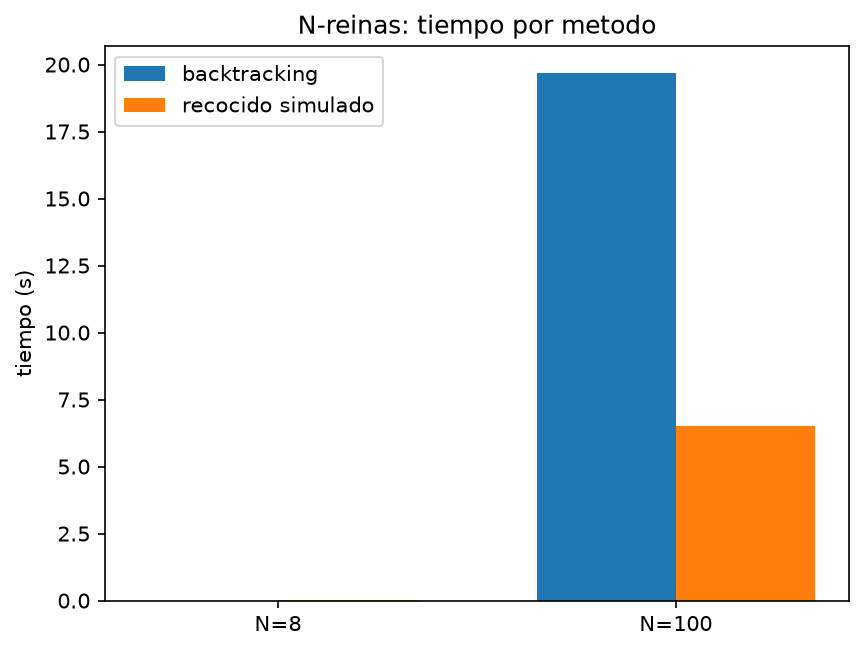
\includegraphics[width=0.62\textwidth]{figures/nqueens_time.png}
\caption{Tiempo de c\'omputo por m\'etodo (\code{experiments/make\_plots.py} sobre
\code{results/tables/nqueens.csv}).}
\label{fig:nqueens-time}
\end{figure}

Como se discuti\'o en \S\ref{sec:impl-csp}, AC-3 de preprocesamiento no cambia el n\'umero
de nodos expandidos en ninguno de los dos tama\~nos -- los dominios de N-reinas ya son
arco-consistentes antes de la primera asignaci\'on. Ambos m\'etodos escalan razonablemente
de $N=8$ a $N=100$ (backtracking: 28 a 159 nodos; recocido simulado: siempre encuentra una
soluci\'on de 0 conflictos dentro del l\'imite de iteraciones/tiempo configurado), y en
$N=100$ el recocido simulado es consistentemente m\'as r\'apido que backtracking exacto
(Figura~\ref{fig:nqueens-time}) -- un resultado esperado, ya que N-reinas tiene
much\'isimas soluciones dispersas por todo el espacio de asignaciones completas, el
r\'egimen exacto donde la b\'usqueda local min-conflicts brilla (ver tambi\'en
Ejercicio~2, \S\ref{sec:ex2}, para el contraste con Sudoku).

\subsection{Todas las soluciones de N-reinas, $N=100$}
\label{sec:app-enum}

El n\'umero real de soluciones de $N$-reinas crece much\'isimo m\'as r\'apido que $N$: el
c\'alculo exacto m\'as grande logrado a la fecha es $N=27$, con m\'as de
$2.34\times10^{17}$ soluciones tras a\~nos de tiempo de CPU acumulado en cl\'usteres
masivos~\cite{oeis000170}. Una enumeraci\'on exhaustiva para $N=100$ es, por lo tanto,
inviable en el tiempo de esta tarea; \code{enumerate\_solutions}
(\code{src/problems/nqueens.py}) corta por \code{max\_solutions} y/o
\code{time\_limit\_seconds} (\code{configs/nqueens.yaml}: 1000 soluciones o 300s, lo que
ocurra primero) y reporta honestamente en \code{stats.extra[\textquotedbl exhaustive\textquotedbl]} si la b\'usqueda
termin\'o sola o fue cortada.

\code{enumerate\_solutions} reutiliza el mismo motor \code{backtrack} de
\S\ref{sec:impl-csp} en modo \code{find\_all=True} (con MRV+LCV+forward checking), en
lugar de una recursi\'on de orden fijo dedicada. Esto importa: con el motor heur\'istico,
la corrida oficial (\code{python experiments/enumerate\_nqueens.py}) explora
\textbf{1{,}213{,}844 nodos en 300s} y encuentra \textbf{1000 soluciones v\'alidas y
distintas} (el tope de \code{max\_solutions}, confirmadas una por una con
\code{is\_valid\_nqueens\_solution}) -- la b\'usqueda se corta por el l\'imite de tiempo, no
porque se agoten las soluciones, as\'i que \code{exhaustive=False} es honesto pero no
indica ninguna dificultad real para \emph{encontrar} soluciones a esta escala.

Esto contrasta fuertemente con un experimento exploratorio (no pedido por el enunciado,
\S7 del notebook) corrido sobre una implementaci\'on \emph{anterior}, con orden fijo de
filas $0,\dots,n-1$ y \textbf{sin} MRV/LCV: dejada corriendo toda una noche en un servidor
remoto con presupuesto de 6 horas, esa versi\'on explor\'o 108{,}119{,}443 nodos y
\textbf{no encontr\'o ninguna soluci\'on}. Esto no es un problema de presupuesto sino el
fen\'omeno de \emph{heavy-tailed runtime} bien documentado en backtracking sin heur\'isticas
de orden~\cite{gomes1997heavytailed}: con un orden determinista fijo, el tiempo hasta la
primera soluci\'on no tiene cota pr\'actica garantizada, y $N=100$ cay\'o del lado
desafortunado para ese orden en particular. La lecci\'on -- y la raz\'on por la que se
reescribi\'o \code{enumerate\_solutions} para reusar el motor con MRV/LCV -- es que la
heur\'istica de orden no solo acelera encontrar \emph{una} soluci\'on
(\S\ref{sec:app-nqueens}), sino que es la diferencia entre una enumeraci\'on que progresa y
una que nunca despega.

\subsection{Coloreado de grafos: 50 y 1000 nodos}
\label{sec:app-coloring}

\textbf{Formulaci\'on CSP} (\code{src/problems/graph\_coloring.py}): variables = v\'ertices;
dominio de cada variable = $\{0,\dots,k-1\}$ para un $k$ dado; restricci\'on: dos v\'ertices
adyacentes no comparten color. \code{problem.neighbors} se llena con la adyacencia real del
grafo, as\'i que AC-3 solo recorre aristas reales ($O(E)$), no todos los pares de
v\'ertices. \textbf{Funci\'on objetivo} de la metaheur\'istica: \code{count\_conflicts},
n\'umero de aristas cuyos dos extremos comparten color; cero es una coloraci\'on v\'alida
con exactamente $k$ colores. Para un $k$ dado, tanto \code{solve\_backtracking} como
\code{solve\_metaheuristic} responden ``¿existe una coloraci\'on v\'alida con exactamente $k$ colores?''; la calidad que compara el enunciado
(``n\'umero de colores'') se obtiene barriendo $k$ de menor a mayor y qued\'andose con el
primero factible.

El formato de entrada/salida sigue exactamente lo que pide el enunciado
(\code{src/utils/graph\_io.py}): la primera l\'inea del archivo de entrada trae
\emph{v\'ertices aristas}, las siguientes \emph{m} l\'ineas son las aristas; la salida
escribe primero el n\'umero de colores usados y luego una l\'inea \emph{color v\'ertice} por
cada v\'ertice.

\subsubsection{50 nodos (\code{gc\_50\_7.txt}): resuelto por completo}

Esta instancia tiene 50 v\'ertices y 865 aristas (densidad 0.706, mucho m\'as densa que un
grafo aleatorio disperso t\'ipico). Antes del barrido oficial, se prob\'o $k$ suelto con
l\'imites de tiempo cortos para entender la estructura del problema (Tabla~\ref{tab:phase}):
para $k\le 7$ el backtracking prueba infactibilidad exhaustivamente r\'apido; para
$k\in[8,13]$ el algoritmo se queda atascado (ni resuelve ni prueba infactibilidad dentro
del l\'imite); para $k\ge14$ resuelve casi instant\'aneamente.

\begin{table}[H]
\centering
\small
\caption{\code{gc\_50\_7.txt}: nodos expandidos por backtracking (FC+AC3+MRV/LCV) seg\'un
$k$, y conflictos finales del recocido simulado con el mismo $k$
(\code{results/tables/graph\_coloring\_k\_sweep.csv}).}
\label{tab:phase}
\begin{tabular}{@{}rrrl@{}}
\toprule
$k$ & Nodos (backtracking) & Conflictos finales (SA) & Backtracking \\
\midrule
7  & 8{,}660   & --  & infactible, probado exhaustivamente (2.95s) \\
10 & 442{,}999 & 14  & timeout a 120s, sin resolver \\
11 & 470{,}644 & 9   & timeout a 120s, sin resolver \\
12 & 533{,}225 & 5   & timeout a 120s, sin resolver \\
13 & 678{,}489 & 2   & timeout a 120s, sin resolver \\
14 & 16{,}214  & 0   & \textbf{resuelto} (2.41s) \\
15 & 51        & 0   & resuelto trivialmente (0.06s) \\
\bottomrule
\end{tabular}
\end{table}

Este patr\'on es el fen\'omeno cl\'asico de \emph{transici\'on de fase} en CSPs: lejos del
umbral (muy restringido o muy holgado), backtracking poda r\'apido en cualquier direcci\'on;
cerca del umbral real de satisfacibilidad, el problema se vuelve computacionalmente duro
tanto para probar factibilidad como infactibilidad~\cite{cheeseman1991hard}. La
Figura~\ref{fig:phase} visualiza esto: el n\'umero de nodos expandidos crece varios
\'ordenes de magnitud al acercarse al umbral desde abajo, y colapsa en cuanto $k$ cruza el
umbral real ($\chi=14$).

\begin{figure}[H]
\centering
\begin{tikzpicture}
\begin{semilogyaxis}[
  width=0.85\textwidth, height=6.2cm,
  xlabel={$k$ (n\'umero de colores permitidos)},
  ylabel={nodos expandidos (escala log)},
  xtick={7,10,11,12,13,14,15},
  grid=major,
  legend pos=north east,
  legend style={font=\scriptsize},
]
\addplot[thick, mark=*, mark options={fill=red}, red] coordinates {(7,8660)};
\addlegendentry{infactible (probado)}
\addplot[thick, mark=square*, mark options={fill=orange}, orange] coordinates {(10,442999) (11,470644) (12,533225) (13,678489)};
\addlegendentry{zona dif\'icil (timeout, 120s)}
\addplot[thick, mark=triangle*, mark options={fill=green!60!black}, green!60!black] coordinates {(14,16214) (15,51)};
\addlegendentry{factible (resuelto)}
\draw[dashed, black!60] (axis cs:13.5,1) -- (axis cs:13.5,900000);
\node[font=\scriptsize, black!60, rotate=90] at (axis cs:13.85,50000) {umbral real $\chi=14$};
\end{semilogyaxis}
\end{tikzpicture}
\caption{Transici\'on de fase en \code{gc\_50\_7.txt}: nodos expandidos por backtracking en
funci\'on de $k$. La dificultad se concentra justo antes del umbral real de
satisfacibilidad~\cite{cheeseman1991hard}.}
\label{fig:phase}
\end{figure}

Con esto, el barrido oficial (\code{configs/graph\_coloring.yaml}, $k\in[10,70]$,
120s por intento) encuentra: \textbf{backtracking, $k=14$} (2.41s, 16{,}214 nodos);
\textbf{recocido simulado, $k=15$} (0.24s) -- la metaheur\'istica no busca el $k$ m\'inimo
por s\'i sola, solo verifica factibilidad para un $k$ dado, as\'i que reporta el primer $k$
del barrido donde converge, no necesariamente el \'optimo (ver \S\ref{sec:app-ortools} para
la confirmaci\'on de que 14 es realmente el m\'inimo).

\subsubsection{1000 nodos (\code{gc\_1000\_9.txt}): acotado, no resuelto por completo}

Esta instancia result\'o mucho m\'as densa de lo que sugiere su nombre: 1000 v\'ertices,
449{,}735 aristas (densidad $0.90$). Un barrido ascendente lineal de $k$ (la misma
estrategia que funcion\'o para 50 nodos) nunca llega a un $k$ factible dentro de un
presupuesto razonable: un clique de tama\~no 49 certifica que $k\le48$ es
\textbf{provablemente infactible} (cota inferior $\chi\ge49$), y una coloraci\'on voraz
(greedy) usa 315 colores como cota superior trivial ($\chi\le315$) -- pero el rango
intermedio completo es, en la pr\'actica, la ``zona dif\'icil'' de la
Figura~\ref{fig:phase} a una escala mucho mayor: ni backtracking ni el recocido simulado
resuelven un solo valor de $k$ en esta zona dentro de minutos.

Ante esto, se recurri\'o a b\'usqueda binaria/galopante contra la ventana
$[48,310]$ usando OR-Tools (CP-SAT) como or\'aculo de factibilidad en cada punto de
prueba (\code{experiments/graph\_coloring\_gallop\_overnight.py}): arrancar desde un punto
ya probado f\'acil ($k=310$, factible) y avanzar hacia abajo con paso que se duplica tras un
\'exito r\'apido y se reduce a la mitad tras cualquier resultado que no lo sea, concentra el
presupuesto de c\'omputo cerca del verdadero umbral en lugar de gastarlo uniformemente. Al
momento de escribir este reporte, el mejor $k$ confirmado factible por esta v\'ia es
$\mathbf{k=302}$ (probado \textsc{OPTIMAL} por CP-SAT). El estado honesto de esta instancia
es entonces:
\begin{equation}
49 \;\le\; \chi(\text{gc\_1000\_9}) \;\le\; 302,
\end{equation}
una ventana a\'un no cerrada. Este es el \'unico rubro de la tarea que no se cierra por
completo (ver \S\ref{sec:app-ortools} para la comparaci\'on de tiempos que motiva esta
decisi\'on, y la Tabla de \S\ref{sec:conclusions} para la postura final). Es, en s\'i mismo,
un resultado leg\'itimo: a esta escala y densidad, ni backtracking exacto con MRV/LCV+FC+AC3
ni recocido simulado de trayectoria \'unica son competitivos frente a un solver CP-SAT
completo como OR-Tools -- precisamente el tipo de brecha que herramientas como
\textsc{Any-CSP} (\S\ref{sec:readings-tonshoff}) intentan cerrar por el lado heur\'istico.

\subsection{Coloreado de grafos vs.\ OR-Tools}
\label{sec:app-ortools}

\code{src/integrations/ortools\_coloring.py} modela ``¿existe coloraci\'on con a lo m\'as $k$ colores?'' como un modelo CP-SAT de OR-Tools (una variable
entera por v\'ertice, restricci\'on \code{color[u] != color[v]} por cada arista) y
\code{find\_min\_colors\_ortools} barre $k$ igual que nuestro propio backtracking, para que
la comparaci\'on sea directa.

\begin{table}[H]
\centering
\small
\caption{Coloreado de grafos: backtracking propio vs.\ recocido simulado propio vs.\
OR-Tools (CP-SAT), mismas instancias (\code{results/tables/coloring\_comparison.csv}).}
\label{tab:coloring-small}
\begin{tabular}{@{}lrrrrrr@{}}
\toprule
Instancia & $V$ & $E$ & $k_{\text{backtracking}}$ & $k_{\text{recocido}}$ & $k_{\text{OR-Tools}}$ & Tiempos (s) BT/SA/OR \\
\midrule
50 nodos   & 50   & 865     & 14 & 15 & 14 & 2.41 / 0.24 / 0.20 \\
1000 nodos & 1000 & 449{,}735 & \multicolumn{3}{c}{ver \S\ref{sec:app-coloring}: $49\le\chi\le302$} & -- \\
\bottomrule
\end{tabular}
\end{table}

\begin{figure}[H]
\centering
\begin{subfigure}[b]{0.48\textwidth}
  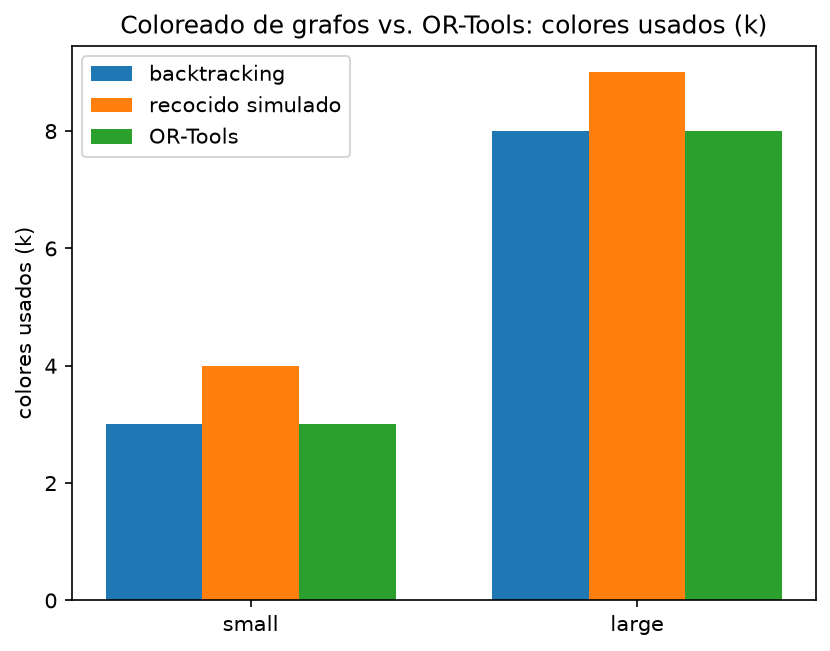
\includegraphics[width=\textwidth]{figures/coloring_comparison_k.png}
  \caption{Colores usados ($k$).}
\end{subfigure}\hfill
\begin{subfigure}[b]{0.48\textwidth}
  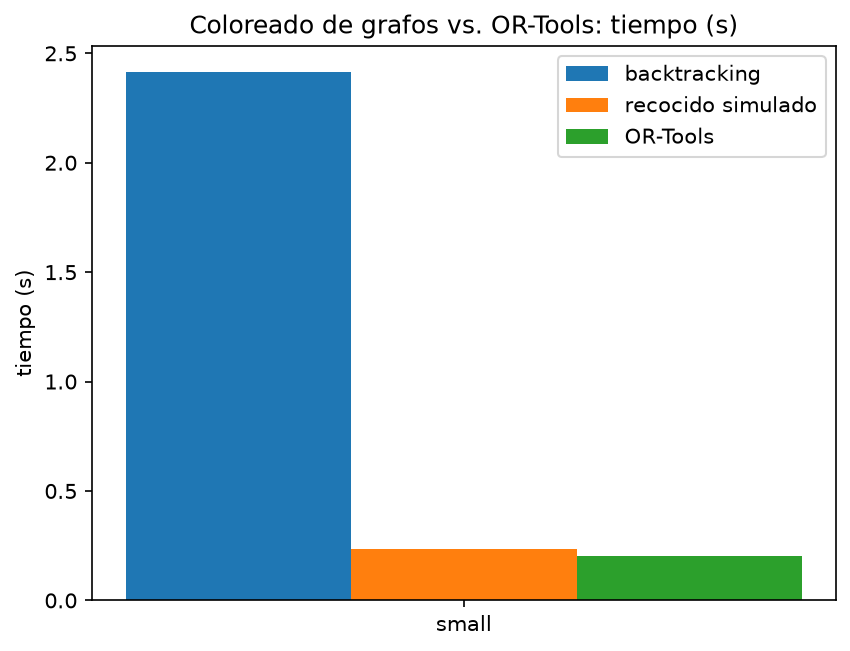
\includegraphics[width=\textwidth]{figures/coloring_comparison_time.png}
  \caption{Tiempo de c\'omputo.}
\end{subfigure}
\caption{Comparaci\'on completa para la instancia de 50 nodos (\code{experiments/make\_plots.py}).}
\label{fig:coloring-comparison}
\end{figure}

\textbf{Lectura}: para el grafo de 50 nodos, backtracking y OR-Tools coinciden en el
\'optimo real ($k=14$) -- OR-Tools es un solver CP-SAT completo y exacto, as\'i que confirma
que 14 es realmente el m\'inimo, no solo lo primero que cada m\'etodo encontr\'o. El
recocido simulado usa un color de m\'as ($k=15$): no busca el $k$ m\'inimo por s\'i mismo,
solo verifica si un $k$ dado es alcanzable sin conflictos. En tiempo, los tres m\'etodos
son comparables en esta escala (0.2--2.4s); la brecha se vuelve dram\'atica en el grafo de
1000 nodos, donde OR-Tools (con horas de c\'omputo distribuidas en b\'usqueda
binaria/galopante) logra confirmar factibilidad en $k=302$ mientras que backtracking y
recocido simulado, en el mismo rango, ni siquiera terminan un solo intento dentro de
minutos -- la ventaja de un solver CP-SAT completo, con propagaci\'on de restricciones
mucho m\'as sofisticada que AC-3+FC, se hace evidente justo donde m\'as importa: cerca del
umbral real de instancias grandes y densas.

\subsection{Gato (\code{gym-tic-tac-toe}) con minimax}
\label{sec:app-tictactoe}

Se model\'o tic-tac-toe como problema de b\'usqueda con adversarios sobre el entorno de
\href{https://github.com/LudwigStumpp/gym-tic-tac-toe}{gym-tic-tac-toe}~\cite{gymtictactoe}
(vendorizado en \code{src/integrations/\_vendor/}): \textsc{Acciones}(s) = casillas libres
de \code{legal\_moves(env)}; \textsc{Resultado}(s,a) = \code{apply\_move} sobre una copia
del entorno (\code{clone\_env}, ya que el tablero es peque\~no y clonar es m\'as simple que
mantener deshacer-movimiento); \textsc{Test-Terminal}(s) = tres en l\'inea o tablero lleno
(\code{is\_terminal}); \textsc{Utilidad}(s) = $+1/-1/0$ como en \S\ref{sec:impl-minimax}.

Se valid\'o con tres pruebas (\code{notebooks/results.ipynb}, secci\'on 6):
\begin{enumerate}[label=\arabic*.]
\item \textbf{minimax vs.\ minimax}: con juego \'optimo de ambos lados, la partida termina
  \textbf{siempre en empate} -- el resultado te\'orico bien conocido de tic-tac-toe, y
  confirmado emp\'iricamente con nuestro propio c\'odigo.
\item \textbf{minimax vs.\ aleatorio, 10 semillas por lado}: un jugador \'optimo
  \textbf{nunca pierde} contra un agente aleatorio, sin importar si juega primero (X) o
  segundo (O).
\item \textbf{Caso a mano, conectado con el Ejercicio~3}: tablero con X en \{0,1\}, O en
  \{3,4\}, turno de X. X puede ganar de inmediato tomando la casilla 2 (completa la fila
  superior): \code{mini\_max(env, X) = 1} y \code{best\_move(env, X) = 2}, como se espera.
\end{enumerate}

Adem\'as, para el Ejercicio~3 (\S\ref{sec:ex3}) se corri\'o \code{mini\_max} sobre el \'arbol
\emph{completo} (sin recorte de profundidad) desde cada uno de los tres primeros
movimientos posibles de X (esquina, borde, centro): los tres dan valor $0$ (empate con
juego \'optimo desde cualquier apertura) -- un contraste \'util con el an\'alisis
heur\'istico de profundidad~2 del Ejercicio~3, que s\'i distingue entre aperturas porque usa
una funci\'on de evaluaci\'on con recorte, no el valor minimax exacto.

% =============================================================================
\section{Ejercicios}
% =============================================================================

Los cuatro ejercicios siguen el planteamiento cl\'asico de CSP y b\'usqueda con
adversarios de Russell y Norvig~\cite{russellnorvig2021}, y se resuelven con las mismas
herramientas conceptuales (formulaci\'on CSP, b\'usqueda local, minimax, poda alfa-beta)
implementadas y aplicadas en las secciones anteriores.

\subsection{Ejercicio 1: $k$ caballos en un tablero $n\times n$}
\label{sec:ex1}

\subsubsection*{(a) Variables}

Un caballo, a diferencia de una casilla, es la entidad que hay que ubicar y de la que hay
exactamente $k$ (dado). Elegimos entonces \textbf{una variable por caballo}:
$$C_1, C_2, \dots, C_k.$$
(La alternativa de usar una variable booleana por casilla, $\{0,1\}^{n^2}$, exigir\'ia
adem\'as una restricci\'on global de cardinalidad ``exactamente $k$ casillas en 1'', menos
natural en el marco de CSP b\'asico que estamos usando en el resto de la tarea; la
formulaci\'on por caballo es, adem\'as, estructuralmente id\'entica a la que usamos para
N-reinas en \S\ref{sec:app-nqueens}: variables = ``piezas'', dominio = casillas.)

\subsubsection*{(b) Dominio}

El dominio de cada $C_i$ es el conjunto de las $n^2$ casillas del tablero:
$$D(C_i) = \{(r,c) : 0\le r\le n-1,\ 0\le c\le n-1\}.$$

\subsubsection*{(c) Restricciones}

Todo \textbf{par} de variables $\{C_i,C_j\}$, $i\neq j$, est\'a restringido (el grafo de
restricciones es completo, igual que en N-reinas) por dos condiciones simult\'aneas:
\begin{enumerate}[label=(\roman*)]
\item \textbf{Distinci\'on}: $C_i \neq C_j$ (dos caballos no pueden ocupar la misma
  casilla).
\item \textbf{No-ataque}: si $C_i=(r_i,c_i)$ y $C_j=(r_j,c_j)$, entonces
  $(|r_i-r_j|,|c_i-c_j|) \notin \{(1,2),(2,1)\}$ (la relaci\'on de movimiento en L de un
  caballo de ajedrez).
\end{enumerate}
Como $k\le n^2$ (dado por el enunciado), el problema siempre tiene al menos la soluci\'on
trivial de casillas suficientes para evitar solaparse, aunque no necesariamente sin
ataques -- eso es lo que la b\'usqueda debe encontrar.

\begin{figure}[H]
\centering
\begin{tikzpicture}[scale=0.75]
  \foreach \x in {0,...,4}{ \foreach \y in {0,...,4}{
    \pgfmathtruncatemacro{\c}{mod(\x+\y,2)}
    \ifnum\c=0 \fill[black!15] (\x,\y) rectangle ++(1,1); \fi
  }}
  \draw[thick] (0,0) rectangle (5,5);
  \foreach \x in {1,...,4}{ \draw (\x,0) -- (\x,5); \draw (0,\x) -- (5,\x); }
  % knights at (row,col): A=(0,0) col0,row0 -> place at bottom-left; B=(1,2); C=(3,3)
  \node[circle,fill=red!70!black,text=white,font=\bfseries,minimum size=0.62cm,inner sep=0pt] (A) at (0.5,0.5) {C};
  \node[circle,fill=red!70!black,text=white,font=\bfseries,minimum size=0.62cm,inner sep=0pt] (B) at (2.5,1.5) {C};
  \node[circle,fill=blue!60!black,text=white,font=\bfseries,minimum size=0.62cm,inner sep=0pt] (D) at (3.5,3.5) {C};
  \draw[-{Latex[length=2mm]}, thick, red!70!black] (A) -- node[above, font=\scriptsize, sloped]{ataque} (B);
  \draw[dashed, thick, blue!60!black] (A) -- node[above, font=\scriptsize, sloped]{sin ataque} (D);
\end{tikzpicture}
\caption{Ejemplo en $5\times5$: los dos caballos rojos se atacan entre s\'i (movimiento en
L, $(|\Delta r|,|\Delta c|)=(1,2)$); el caballo azul no ataca al caballo rojo inferior
($(|\Delta r|,|\Delta c|)=(3,3)$).}
\label{fig:knights}
\end{figure}

\subsubsection*{(d) Variante de optimizaci\'on: m\'aximo n\'umero de caballos, con b\'usqueda local}

Aqu\'i $k$ ya no est\'a dado -- se busca \emph{maximizar} el n\'umero de caballos sin
ataques, el an\'alogo de un conjunto independiente m\'aximo en el ``grafo de ataque'' del
caballo. Formulamos esto como b\'usqueda local sobre asignaciones completas (en el
esp\'iritu de min-conflicts, \S\ref{sec:impl-sa}), no sobre asignaciones parciales:

\begin{itemize}[leftmargin=1.4em]
\item \textbf{Estado}: un subconjunto $S\subseteq\{0,\dots,n-1\}^2$ de casillas ocupadas
  por caballos (no necesariamente $k$; el tama\~no de $S$ es parte de lo que se optimiza).
\item \textsc{Acciones}$(s)$: $\{\textsc{Agregar}(casilla) : \text{casilla}\notin S\} \cup
  \{\textsc{Quitar}(casilla) : \text{casilla}\in S\}$ -- agregar o quitar un caballo de una
  casilla vac\'ia/ocupada. (Tambi\'en se puede permitir \textsc{Mover}(casilla$_1$,
  casilla$_2$) como acci\'on compuesta, \'util para escapar \'optimos locales sin cambiar el
  conteo actual de caballos.)
\item \textsc{Resultado}$(s,a)$: el conjunto $S$ tras aplicar la acci\'on (agregar, quitar
  o mover una casilla).
\item \textbf{Funci\'on objetivo} (a maximizar):
  $$f(s) = |S| \;-\; M\cdot\text{conflictos}(s),$$
  donde $\text{conflictos}(s)$ es el n\'umero de pares de caballos en $S$ que se atacan
  (exactamente el mismo tipo de funci\'on que \code{count\_conflicts} en
  \S\ref{sec:impl-sa}, aplicada aqu\'i al grafo de ataque del caballo en vez de al grafo de
  N-reinas o de coloreado) y $M$ es una constante lo bastante grande (p.\,ej.\ $M>n^2$)
  para garantizar que \emph{cualquier} reducci\'on de un conflicto vale m\'as que agregar
  un caballo adicional -- as\'i, ascenso de colinas o recocido simulado sobre $f$
  primero se ve empujado hacia estados sin conflictos, y una vez ah\'i, hacia agregar m\'as
  caballos.
\end{itemize}

Una alternativa m\'as simple -- restringir el espacio de estados a solo configuraciones
\emph{sin conflictos} y usar $\textsc{Acciones}(s)=\{\textsc{Agregar}(c) : c\notin S,\ S\cup\{c\}
\text{ sigue sin conflictos}\}$, maximizando directamente $|S|$ -- es m\'as f\'acil de
implementar (ascenso de colinas voraz puro) pero se estanca en un m\'aximo \emph{local}: un
conjunto independiente \emph{maximal} pero no necesariamente \emph{m\'aximo} (no se puede
agregar ning\'un caballo m\'as sin conflicto, pero existe otra configuraci\'on con m\'as
caballos en total). Permitir temporalmente estados con conflictos, v\'ia la funci\'on
objetivo penalizada de arriba y una metaheur\'istica como recocido simulado que acepta
movimientos que empeoran $f$ con probabilidad decreciente, es precisamente el mecanismo
que nos permite salir de esos \'optimos locales -- la misma raz\'on de ser del
Metropolis-accept en \S\ref{sec:impl-sa}.

\subsection{Ejercicio 2: Sudoku con b\'usqueda local}
\label{sec:ex2}

La pregunta es c\'omo le ir\'ia a un solucionador de b\'usqueda local (tipo min-conflicts,
sobre asignaciones \emph{completas}, an\'alogo exacto de nuestro recocido simulado en
\S\ref{sec:impl-sa}) usando como heur\'istica minimizar el n\'umero de restricciones
violadas.

\textbf{Respuesta: muy mal}, y la raz\'on es estructural, no de implementaci\'on. Min-conflicts
funciona extraordinariamente bien en N-reinas (\S\ref{sec:app-nqueens}) porque N-reinas
tiene una estructura muy particular: el espacio de asignaciones completas es enorme, pero
tambi\'en lo es la \emph{densidad relativa} de soluciones dentro de \'el (para $N$ grande,
hay much\'isimas soluciones dispersas por todo el espacio), y el paisaje de ``n\'umero de
conflictos'' tiene, emp\'iricamente, pocos m\'inimos locales profundos en relaci\'on al
tama\~no del espacio -- casi cualquier asignaci\'on aleatoria tiene un camino de descenso
corto hacia alg\'una soluci\'on.

Sudoku es casi lo opuesto en ambos ejes:
\begin{itemize}[leftmargin=1.4em]
\item \textbf{Muy pocas soluciones, o una sola}: un Sudoku bien planteado tiene
  t\'ipicamente \emph{una \'unica} soluci\'on entre un espacio combinatorio de asignaciones
  completas igual de gigante. La ``aguja en el pajar'' es much\'isimo m\'as dif\'icil de
  encontrar por descenso de gradiente que cuando hay millones de agujas repartidas por
  todo el pajar.
\item \textbf{Restricciones mucho m\'as densas y locales}: cada celda participa en tres
  grupos de restricci\'on (fila, columna, caja $3\times3$) con 20 vecinos distintos en
  total, contra 2 tipos de restricci\'on (fila/diagonal) por reina en N-reinas con un
  grafo de restricciones igual de denso pero mucho m\'as flexible en soluciones. Esta
  densidad hace que casi cualquier asignaci\'on completa aleatoria quede muy lejos (en
  n\'umero de conflictos) de \emph{cualquier} soluci\'on v\'alida, y que el paisaje de
  conflictos tenga much\'isimos m\'inimos locales profundos -- mesetas anchas donde ning\'un
  movimiento de una sola celda reduce el conteo de violaciones, pero que no son la
  soluci\'on.
\item \textbf{Las pistas dadas reducen los grados de libertad efectivos}: en un Sudoku con
  muchas celdas ya fijas, las pocas celdas libres est\'an fuertemente acopladas entre s\'i
  (cambiar una casi siempre exige cambiar varias m\'as para no violar otra restricci\'on),
  as\'i que el movimiento ``mover una celda a la vez'' de min-conflicts rara vez encuentra
  una direcci\'on de mejora real.
\end{itemize}

En la pr\'actica (y esto es adem\'as un resultado conocido en la literatura de CSP), un
solucionador de b\'usqueda local con esta heur\'istica resuelve Sudokus \emph{f\'aciles}
(pocas pistas, muchos grados de libertad) de forma aceptable, pero su tasa de \'exito cae
dr\'asticamente en Sudokus dif\'iciles y se estanca con frecuencia en asignaciones con
varias restricciones a\'un violadas, muy lejos de la soluci\'on \'unica -- exactamente lo
opuesto al comportamiento robusto que observamos para nuestro propio recocido simulado en
N-reinas $N=100$ (\S\ref{sec:app-nqueens}), donde siempre converge a 0 conflictos. Es un
buen contraejemplo de que min-conflicts ``simplemente funciona bien'' para CSPs en
general: funciona bien quando la estructura del problema lo favorece, y Sudoku es
precisamente el caso donde no.

\subsection{Ejercicio 3: \'arbol de juego del gato}
\label{sec:ex3}

Se usa la numeraci\'on de casillas
$\begin{smallmatrix}1&2&3\\4&5&6\\7&8&9\end{smallmatrix}$
(filas $\{1,2,3\},\{4,5,6\},\{7,8,9\}$; columnas $\{1,4,7\},\{2,5,8\},\{3,6,9\}$;
diagonales $\{1,5,9\},\{3,5,7\}$).

\subsubsection*{(a) N\'umero aproximado de partidas posibles}

Una cota superior ingenua es $9!=362{,}880$ (todas las formas de llenar el tablero en
secuencia, ignorando que el juego termina en cuanto alguien gana). Contando correctamente
que la partida se detiene apenas hay tres en l\'inea, el n\'umero real de partidas
distintas (secuencias de movimientos) es menor: la cifra com\'unmente citada es
\textbf{$\approx 255{,}168$} partidas posibles. (Vale la pena distinguir esto del n\'umero
de \emph{posiciones} de tablero alcanzables, que es much\'isimo menor: 5{,}478 posiciones
legales, o 138 si se identifican posiciones sim\'etricas entre s\'i -- una partida es una
secuencia de movimientos, no solo el tablero final.)

\subsubsection*{(b) \'Arbol completo hasta profundidad 2, con simetr\'ia}

Por simetr\'ia del tablero vac\'io (grupo diedral $D_4$, orden 8), el primer movimiento de
X tiene solo \textbf{3 clases distintas}: esquina, borde (centro de lado) y centro. Para
cada clase, la simetr\'ia restante (la que deja fija la casilla de X) punt\'ua las
respuestas posibles de O en clases m\'as finas:

\begin{itemize}[leftmargin=1.4em]
\item \textbf{X en esquina} (p.\,ej.\ casilla 1): la \'unica simetr\'ia que sobrevive es la
  reflexi\'on sobre la diagonal 1-5-9. Las 8 casillas restantes se agrupan en
  \textbf{5 clases}: centro (5), esquina opuesta (9), esquina adyacente
  ($\{3,7\}$), borde adyacente a la esquina de X ($\{2,4\}$), borde lejano
  ($\{6,8\}$).
\item \textbf{X en borde} (p.\,ej.\ casilla 2): sobrevive la reflexi\'on vertical. Las 8
  casillas restantes se agrupan en \textbf{5 clases}: centro (5), borde opuesto (8),
  esquina cercana ($\{1,3\}$), esquina lejana ($\{7,9\}$), borde-lado ($\{4,6\}$).
\item \textbf{X en centro} (casilla 5): sobrevive el grupo $D_4$ completo. Las 8 casillas
  restantes se agrupan en solo \textbf{2 clases}: esquina ($\{1,3,7,9\}$) o borde
  ($\{2,4,6,8\}$).
\end{itemize}

En total, profundidad~2 tiene $5+5+2=\mathbf{12}$ posiciones distintas bajo simetr\'ia (no
$9\times8=72$), como se ilustra en la Figura~\ref{fig:tictactoe-tree}.

\subsubsection*{(c) Evaluaciones en profundidad 2}

Ninguna posici\'on de profundidad~2 es terminal (solo hay 2 marcas en el tablero), as\'i
que se punt\'ua con $\text{Eval}(s)=3X_2(s)+X_1(s)-\big(3O_2(s)+O_1(s)\big)$. Los 12 valores
(deducidos directamente de la definici\'on de $X_n,O_n$, contando l\'ineas -- filas,
columnas o diagonales -- con exactamente $n$ marcas de un jugador y ninguna del otro) se
muestran junto al \'arbol en la Figura~\ref{fig:tictactoe-tree}.

\subsubsection*{(d) Propagaci\'on minimax a profundidad 1 y 0}

Tratando los 12 valores de Eval de (c) como si fueran los valores terminales de un \'arbol
cortado en profundidad~2 (minimax con recorte de profundidad, id\'entico en esp\'iritu a
usar una funci\'on de evaluaci\'on heur\'istica cuando el \'arbol real es demasiado grande
para resolver exactamente -- aqu\'i se hace por pedagog\'ia, ya que el \'arbol real de
tic-tac-toe s\'i cabe completo, ver el recuadro de verificaci\'on m\'as abajo), los nodos de
profundidad~1 (turno de O, nodo MIN) toman el m\'inimo de sus hijos, y la ra\'iz (turno de
X, nodo MAX) toma el m\'aximo de los tres:
\begin{align*}
\text{profundidad 1:}\quad & \text{esquina}=\min\{-1,0,0,1,1\}=-1, \\
                            & \text{borde}=\min\{-2,-1,-1,0,0\}=-2, \\
                            & \text{centro}=\min\{1,2\}=1 \\[4pt]
\text{ra\'iz}\ (\text{profundidad 0):}\quad & \max\{-1,-2,1\} = \boxed{1},\ \text{alcanzado jugando \textbf{el centro}.}
\end{align*}
Bajo este an\'alisis heur\'istico de profundidad~2, \textbf{la mejor primera jugada para X
es el centro} -- consistente con la sabidur\'ia est\'andar de tic-tac-toe (el centro es la
apertura m\'as fuerte en la pr\'actica) y con que, dentro de esa rama, la mejor respuesta de
O es una esquina (valor 1) y no un borde (valor 2, un error conocido de O).

\begin{quotation}
\noindent\small\textbf{Verificaci\'on con nuestro propio c\'odigo (\S\ref{sec:app-tictactoe})}: al
correr \code{mini\_max} \emph{sin} recorte de profundidad (el \'arbol completo real, no la
funci\'on Eval) desde cada apertura, las tres dan valor $0$ -- las tres son partidas
empatadas con juego \'optimo, incluyendo el borde. Esto no contradice (d): Eval es una
heur\'istica de recorte a profundidad~2 y, como toda heur\'istica, puede preferir una
jugada sobre otra aunque el valor minimax exacto (a profundidad completa) las empate; de
hecho ilustra bien \emph{por qu\'e} se necesitan funciones de evaluaci\'on razonables
cuando explorar el \'arbol completo no es viable (tableros m\'as grandes, ajedrez, etc.):
capturan buenas heur\'isticas (``el centro es fuerte'') incluso sin resolver el juego por
completo.
\end{quotation}

\subsubsection*{(e) Nodos podados por poda alfa-beta con orden \'optimo}

Con orden \'optimo (en cada nodo MIN, explorar primero el hijo de menor valor; en el nodo
MAX ra\'iz, explorar primero el hijo de mayor valor), simulamos alfa-beta sobre el mismo
\'arbol:
\begin{itemize}[leftmargin=1.4em]
\item La ra\'iz explora primero \textbf{centro} (el de mayor valor, 1): sin cota a\'un
  ($\alpha=-\infty$), se eval\'uan sus 2 hijos completos (1 y 2); $\alpha$ sube a 1.
\item Rama \textbf{esquina}: su primer hijo en orden \'optimo es \emph{centro} (valor
  $-1$). Como $-1\le\alpha(1)$, el nodo MIN ``esquina'' ya no puede superar 1
  -- se \textbf{podan sus otros 4 hijos} (esquina opuesta, esquina adyacente, borde
  adyacente, borde lejano).
\item Rama \textbf{borde}: su primer hijo en orden \'optimo es \emph{centro} (valor
  $-2$). Como $-2\le\alpha(1)$, se \textbf{podan sus otros 4 hijos} (borde opuesto,
  esquina cercana, esquina lejana, borde-lado).
\end{itemize}
En total se eval\'uan solo \textbf{4 de los 12} nodos de profundidad~2 (los dos hijos de
``centro'', m\'as el hijo ``centro'' de cada una de las otras dos ramas); los
\textbf{8 restantes} se podan, como se marca con c\'irculos punteados en la
Figura~\ref{fig:tictactoe-tree}.

\begin{figure}[H]
\centering
\resizebox{\textwidth}{!}{%
\begin{tikzpicture}[
  every node/.style={font=\small},
  leaf/.style={draw, rounded corners=2pt, fill=white, inner sep=2pt, align=center, text width=1.7cm},
  mid/.style={draw, rounded corners=2pt, fill=blue!8, inner sep=4pt, align=center},
  rootstyle/.style={draw, rounded corners=2pt, fill=blue!18, inner sep=5pt, very thick, align=center},
]
% ---------------- depth 2 leaves: coordinates ----------------
% corner group (x=0,2.0,4.0,6.0,8.0), edge group, center group
\node[leaf] (c1) at (0,0)   {\tttboard{X}{}{}{}{O}{}{}{}{} \\[1pt] \scriptsize (a) centro $-1$};
\node[leaf] (c2) at (2.0,0) {\tttboard{X}{}{}{}{}{}{}{}{O} \\[1pt] \scriptsize (b) esq.\ op.\ $0$};
\node[leaf] (c3) at (4.0,0) {\tttboard{X}{}{O}{}{}{}{}{}{} \\[1pt] \scriptsize (c) esq.\ ady.\ $0$};
\node[leaf] (c4) at (6.0,0) {\tttboard{X}{O}{}{}{}{}{}{}{} \\[1pt] \scriptsize (d) b.\ ady.\ $1$};
\node[leaf] (c5) at (8.0,0) {\tttboard{X}{}{}{}{}{O}{}{}{} \\[1pt] \scriptsize (e) b.\ lej.\ $1$};

\node[leaf] (e1) at (10.8,0) {\tttboard{}{X}{}{}{O}{}{}{}{} \\[1pt] \scriptsize (f) centro $-2$};
\node[leaf] (e2) at (12.8,0) {\tttboard{}{X}{}{}{}{}{}{O}{} \\[1pt] \scriptsize (g) op.\ $0$};
\node[leaf] (e3) at (14.8,0) {\tttboard{O}{X}{}{}{}{}{}{}{} \\[1pt] \scriptsize (h) esq.\ cer.\ $-1$};
\node[leaf] (e4) at (16.8,0) {\tttboard{}{X}{}{}{}{}{O}{}{} \\[1pt] \scriptsize (i) esq.\ lej.\ $-1$};
\node[leaf] (e5) at (18.8,0) {\tttboard{}{X}{}{O}{}{}{}{}{} \\[1pt] \scriptsize (j) lado $0$};

\node[leaf] (m1) at (21.6,0) {\tttboard{O}{}{}{}{X}{}{}{}{} \\[1pt] \scriptsize (k) esquina $1$};
\node[leaf] (m2) at (23.6,0) {\tttboard{}{O}{}{}{X}{}{}{}{} \\[1pt] \scriptsize (l) borde $2$};

% pruned ellipses, ajustadas autom\'aticamente al tama\~no real de cada nodo
\foreach \n in {c2,c3,c4,c5,e2,e3,e4,e5}{
  \node[draw=red, thick, dashed, ellipse, fit=(\n), inner sep=1pt] {};
}

% ---------------- depth 1 ----------------
\node[mid] (D1c) at (4.0,3.4)  {esquina \\ $\min=-1$};
\node[mid] (D1e) at (14.8,3.4) {borde \\ $\min=-2$};
\node[mid] (D1m) at (22.6,3.4) {centro \\ $\min=1$};

\foreach \c in {c1,c2,c3,c4,c5} \draw[black!50] (D1c) -- (\c);
\foreach \c in {e1,e2,e3,e4,e5} \draw[black!50] (D1e) -- (\c);
\foreach \c in {m1,m2} \draw[black!50] (D1m) -- (\c);

% ---------------- depth 0 ----------------
\node[rootstyle] (root) at (13.3,6.8) {tablero vac\'io \\ $\max=1$ (jugar \textbf{centro})};
\draw[black!50] (root) -- (D1c);
\draw[black!50] (root) -- (D1e);
\draw[very thick, blue] (root) -- (D1m);

\node[font=\scriptsize\itshape, black!55] at (13.3,-2.1) {\'ovalos punteados = podados por poda alfa-beta con orden \'optimo (parte e); rama azul = mejor jugada (parte d)};
\end{tikzpicture}%
}
\caption{\'Arbol de juego del gato hasta profundidad 2, reducido por simetr\'ia (3 nodos en
profundidad 1, 12 en profundidad 2, etiquetados (a)--(l)). Cada hoja muestra
$\text{Eval}(s)$ (parte c); los nodos intermedios y la ra\'iz muestran el valor minimax
propagado (parte d); los \'ovalos punteados marcan los nodos que la poda alfa-beta con
orden \'optimo no necesita evaluar (parte e).}
\label{fig:tictactoe-tree}
\end{figure}

\subsection{Ejercicio 4: correctud de la poda alfa-beta}
\label{sec:ex4}

\textbf{Notaci\'on.} Sea $n_1$ el nodo ra\'iz bajo estudio (tipo MIN) y sea $n_1, n_2,
\dots, n_j$ una cadena de nodos donde $n_{i+1}$ es \emph{un} hijo de $n_i$ (el que est\'a en
el camino hacia $n_j$), alternando tipo: $n_i$ es MIN si $i$ es impar y MAX si $i$ es par
(as\'i, $n_j$ MAX $\Rightarrow j$ par). En cada nivel $i\ge2$, escribimos los \textbf{dem\'as}
hijos de $n_{i-1}$ (los hermanos de $n_i$) separados en dos grupos, siguiendo la
definici\'on del enunciado:
\begin{itemize}[leftmargin=1.4em]
\item $l_i$ = valor extremo (m\'inimo si $n_{i-1}$ es MIN, m\'aximo si $n_{i-1}$ es MAX) de
  los hermanos de $n_i$ que est\'an a su \textbf{izquierda} y cuyo valor minimax
  \textbf{ya se conoce} (fueron explorados primero, en b\'usqueda de izquierda a derecha).
\item $r_i$ = el mismo extremo, pero de los hermanos de $n_i$ que est\'an a su
  \textbf{derecha} y \textbf{a\'un no se han explorado} (valor desconocido por ahora).
\end{itemize}
Con esta notaci\'on, $n_1=\min(n_2,n_{2,1},\dots,n_{2,b_2})$ del enunciado se reescribe
como $n_1 = \min(l_2,\, n_2,\, r_2)$, donde $l_2$ y $r_2$ resumen colectivamente a los
dem\'as $b_2-1$ hijos de $n_1$.

\subsubsection*{(a) Expresi\'on de $n_1$ en t\'erminos de $n_3$ (patr\'on base)}

An\'alogamente, $n_2$ (nodo MAX) se expresa en t\'erminos de \emph{su} hijo en el camino,
$n_3$, y los hermanos de \'este:
$$n_2 = \max(l_3,\, n_3,\, r_3).$$
Sustituyendo en $n_1=\min(l_2,n_2,r_2)$:
$$
n_1 = \min\big(l_2,\ \max(l_3, n_3, r_3),\ r_2\big).
$$
Esto expresa $n_1$ en t\'erminos de $n_3$ (el nieto de $n_1$ en el camino hacia $n_j$) y de
los valores $l_2,r_2,l_3,r_3$ de los hermanos encontrados en el camino.

\subsubsection*{(b) Generalizaci\'on a $n_j$ arbitrario, en t\'erminos de $l_i,r_i$}

Repitiendo la sustituci\'on nivel a nivel hasta llegar a $n_j$ (es decir, sustituyendo
$n_{i-1}=\text{op}_{i-1}(l_i,n_i,r_i)$ para $i=2,3,\dots,j$, con $\text{op}_{i-1}=\min$ si
$n_{i-1}$ es MIN y $\max$ si es MAX):
$$
n_1 = \min\Big(l_2,\ \max\big(l_3,\ \min(l_4,\ \max(l_5,\ \dots,\ \text{op}_{j-1}(l_j,n_j,r_j)\dots,\,r_4),\,r_3\big),\,r_2\Big).
$$
Es decir, $n_1$ queda escrito como una torre de $\min/\max$ anidados que alterna con la
profundidad, con $n_j$ en el centro y un par $(l_i,r_i)$ a cada nivel intermedio.

\subsubsection*{(c) Cota sobre $n_j$ (caso $n_j$ nodo MAX, $j$ par) para que afecte a $n_1$}

Usamos un \'unico hecho, v\'alido para \emph{cualquier} argumento de $\min$ o de $\max$:
\textbf{tanto $\min$ como $\max$ son funciones mon\'otonas no decrecientes en cada uno de
sus argumentos.} En particular, para el nivel inmediatamente superior a $n_j$ (que es
MIN, ya que $n_j$ es MAX): $n_{j-1}=\min(l_j,n_j,r_j)$, y por definici\'on de m\'inimo,
$$
n_{j-1}\le l_j \quad\text{para \emph{cualquier} valor de }n_j.
$$
M\'as a\'un, si $n_j \ge l_j$, entonces $\min(l_j,n_j,r_j)=\min(l_j,r_j)$
\textbf{no depende del valor exacto de $n_j$} (aumentar $n_j$ por encima de $l_j$ nunca
cambia qui\'en gana el m\'inimo). Por monoton\'ia, ese mismo valor $n_{j-1}$ se propaga hacia
arriba sin que $n_1$ dependa de $n_j$ una vez que $n_{j-1}$ dej\'o de depender de \'el.
Subiendo el argumento un nivel m\'as (por monoton\'ia de $\max$ en $n_{j-2}=\max(l_{j-1},
n_{j-1},r_{j-1})$, y as\'i sucesivamente): mientras $n_{j-1}\le l_j$ no cambie, ninguno de
los ancestros de $n_j$ cambia tampoco. Concretamente, con b\'usqueda de izquierda a
derecha (los $l_i$ ya conocidos en cada nivel MIN entre $n_1$ y $n_j$ son exactamente las
cotas $\alpha$ que un ancestro MAX ya garantiz\'o), la condici\'on para que $n_j$ sea
\textbf{irrelevante} para $n_1$ es
$$
\boxed{\,n_j \ge \alpha := \max\{\, l_i : n_{i-1}\text{ es un nodo MIN},\ 2\le i\le j\,\}\,}
$$
es decir, en cuanto se descubre (sin necesidad de conocer su valor exacto, basta una cota
inferior) que $n_j \ge \alpha$, se puede \textbf{podar} el resto de los hijos a\'un no
explorados de $n_j$ (y de sus hermanos futuros) sin riesgo de cambiar $n_1$: $\alpha$ es
precisamente el mejor valor que un ancestro MIN de $n_j$ ya ten\'ia garantizado por otro
camino, as\'i que un $n_j$ que ya lo iguala o supera no puede mejorar la situaci\'on del
jugador MIN en $n_{j-1}$.

\subsubsection*{(d) Caso sim\'etrico: $n_j$ nodo MIN}

Si en cambio $n_j$ es un nodo MIN ($j$ impar), su padre $n_{j-1}$ es MAX:
$n_{j-1}=\max(l_j,n_j,r_j)$, y por la misma monoton\'ia, $n_{j-1}\ge l_j$ para cualquier
valor de $n_j$; si $n_j\le l_j$, entonces $\max(l_j,n_j,r_j)=\max(l_j,r_j)$ ya no depende
de $n_j$. Propagando igual que en (c), la condici\'on para podar el resto del subarbol de
$n_j$ sin riesgo es
$$
\boxed{\,n_j \le \beta := \min\{\, l_i : n_{i-1}\text{ es un nodo MAX},\ 2\le i\le j\,\}\,}
$$
el an\'alogo exacto de (c) intercambiando los roles de MIN y MAX -- $\beta$ es la cota que
en la literatura est\'andar se llama \emph{beta} (el mejor valor que un ancestro MAX ya
tiene garantizado), mientras que la $\alpha$ de la parte (c) es la cota \emph{alfa}
(el mejor valor que un ancestro MIN ya tiene garantizado). Esto es exactamente la poda
alfa-beta: en un nodo MAX se poda si su valor parcial ya alcanza o supera $\beta$
(``poda beta''); en un nodo MIN se poda si su valor parcial ya alcanza o queda por debajo
de $\alpha$ (``poda alfa'').

\begin{figure}[H]
\centering
\begin{tikzpicture}[
  node distance=1.35cm and 1.9cm,
  every node/.style={font=\small},
  nd/.style={draw, circle, minimum size=0.9cm, inner sep=0pt, align=center},
  sib/.style={draw, rounded corners=1pt, fill=black!5, font=\scriptsize, inner sep=2pt, align=center},
]
\node[nd] (n1) {$n_1$\\ \tiny MIN};
\node[sib, left=of n1] (l2) {$l_2$};
\node[sib, right=of n1] (r2) {$r_2$};
\node[nd, below=of n1] (n2) {$n_2$\\ \tiny MAX};
\node[sib, left=of n2] (l3) {$l_3$};
\node[sib, right=of n2] (r3) {$r_3$};
\node[nd, below=of n2] (n3) {$n_3$\\ \tiny MIN};
\node[font=\scriptsize\itshape] (dots) [below=0.55cm of n3] {$\vdots$};
\node[nd, below=1.55cm of n3] (nj) {$n_j$\\ \tiny MAX};
\node[sib, left=of nj] (lj) {$l_j$};
\node[sib, right=of nj] (rj) {$r_j$ \\ \tiny (¿?)};

\draw (n1) -- (l2); \draw (n1) -- (r2); \draw[very thick] (n1) -- (n2);
\draw (n2) -- (l3); \draw (n2) -- (r3); \draw[very thick] (n2) -- (n3);
\draw[very thick, dashed] (n3) -- (dots);
\draw[very thick, dashed] (dots) -- (nj);
\draw (nj) -- (lj); \draw (nj) -- (rj);

\node[font=\scriptsize, black!55, align=left] at (4.6,-1.5) {camino $n_1\to n_j$ en negritas;\\ $l_i$ = hermanos izq.\ (conocidos);\\ $r_i$ = hermanos der.\ (a\'un sin explorar)};
\end{tikzpicture}
\caption{Notaci\'on usada en el Ejercicio~4: cadena $n_1,\dots,n_j$ alternando MIN/MAX, con
los valores $l_i$ (hermanos izquierdos, ya conocidos) y $r_i$ (hermanos derechos, a\'un no
explorados) en cada nivel.}
\label{fig:alphabeta-proof}
\end{figure}

% =============================================================================
\section{Reproducibilidad}
\label{sec:repro}
% =============================================================================

El c\'odigo completo, con instrucciones detalladas de instalaci\'on y ejecuci\'on de cada
experimento, vive en el repositorio (\code{README.md}). En resumen:

\begin{lstlisting}[language=bash, caption={Reproducci\'on de todos los resultados de este reporte.}]
python3 -m venv .venv && source .venv/bin/activate
pip install -r requirements.txt

pytest                                     # 13 pruebas unitarias, todas pasan
python experiments/run_nqueens.py          # N=8 y N=100: backtracking + recocido simulado
python experiments/enumerate_nqueens.py    # todas las soluciones de N=100 (acotado)
python experiments/run_graph_coloring.py   # 50 y 1000 nodos: backtracking + recocido simulado
python experiments/compare_coloring.py     # + comparacion contra OR-Tools
python experiments/make_plots.py           # genera report/figures/*.png
\end{lstlisting}

Los grafos de 50/1000 nodos usados son los provistos para la tarea
(\code{data/graphs/gc\_50\_7.txt}, \code{gc\_1000\_9.txt}), le\'idos y escritos en el
formato exacto que pide el enunciado (primera l\'inea: v\'ertices y aristas; salida:
n\'umero de colores y despu\'es \emph{color v\'ertice} por l\'inea) v\'ia
\code{src/utils/graph\_io.py}. La b\'usqueda del umbral real de \code{gc\_1000\_9.txt}
(\S\ref{sec:app-coloring}) corri\'o en un servidor remoto por las horas de c\'omputo
involucradas; los scripts correspondientes (\code{experiments/graph\_coloring\_*\_overnight.py})
tambi\'en est\'an en el repositorio, documentados en \code{README.md}.

% =============================================================================
\section{Conclusiones}
\label{sec:conclusions}
% =============================================================================

Backtracking exacto (con MRV+LCV+forward checking) y recocido simulado resultaron
complementarios, no intercambiables: backtracking siempre certifica correctud (o
infactibilidad, si AC-3 vac\'ia un dominio) pero paga un costo exponencial en el peor
caso; recocido simulado no certifica nada (no distingue ``no hay soluci\'on con este $k$''
de ``no la encontr\'e a tiempo'') pero escala much\'isimo mejor en problemas con muchas
soluciones dispersas (N-reinas) y es competitivo en tiempo incluso cuando encuentra un $k$
subóptimo (coloreado de 50 nodos). AC-3 como preprocesamiento puro, en ambos problemas
aplicados aqu\'i, no aport\'o poda adicional sobre FC+MRV/LCV -- su valor real habr\'ia
estado en usarlo como MAC durante la b\'usqueda, no antes de que empiece.

La comparaci\'on m\'as reveladora fue contra OR-Tools: en la instancia peque\~na (50
nodos) los tres m\'etodos coinciden en tiempo y calidad; en la instancia grande y densa
(1000 nodos, densidad 0.90) OR-Tools -- un solver CP-SAT completo con propagaci\'on de
restricciones mucho m\'as sofisticada que AC-3+FC -- es el \'unico de los tres capaz de
progresar en un tiempo razonable, mientras que backtracking y recocido simulado propios ni
siquiera terminan un intento. Esto no es una falla de la implementaci\'on sino una
ilustraci\'on directa, con datos propios, del fen\'omeno de transici\'on de fase en
CSPs~\cite{cheeseman1991hard} a una escala donde herramientas artesanales (por bien
implementadas que est\'en) dejan de ser competitivas frente a un solver industrial, y de
por qu\'e propuestas como \textsc{Any-CSP}~\cite{tonshoff2023onemodel}
(\S\ref{sec:readings-tonshoff}) tienen sentido como complemento heur\'istico en ese
r\'egimen.

De las lecturas, la conexi\'on m\'as directa con lo implementado fue la de Doerr et
al.~\cite{doerr2024runtime} (\S\ref{sec:readings-doerr}): nuestro recocido simulado es una
b\'usqueda de \emph{una sola trayectoria}, y la \'unica corrida (de 18) que no convergi\'o en
la exploraci\'on de schedulers fue justamente la m\'as parecida a quedarse sin mecanismo
para escapar un m\'inimo casi alcanzado. La evidencia te\'orica de que la diversidad
poblacional ofrece garant\'ias demostrables de mejora sugiere que, si se tuviera que
seguir iterando sobre este proyecto, un algoritmo gen\'etico (la tercera opci\'on de
metaheur\'istica que permit\'ia el enunciado) ser\'ia un candidato natural para atacar
justamente el caso a\'un abierto de esta tarea: cerrar el n\'umero crom\'atico de
\code{gc\_1000\_9.txt}.

% =============================================================================
\begin{thebibliography}{99}

\bibitem{tonshoff2023onemodel}
T\"onshoff, J., Kisin, B., Lindner, J., \& Grohe, M. (2023).
\emph{One Model, Any CSP: Graph Neural Networks as Fast Global Search Heuristics for
Constraint Satisfaction}. Proceedings of the Thirty-Second International Joint Conference
on Artificial Intelligence (IJCAI-23), pp.~4280--4288.

\bibitem{doerr2024runtime}
Doerr, B., Echarghaoui, A., Jamal, M., \& Krejca, M.~S. (2024).
\emph{Runtime Analysis of the $(\mu+1)$ GA: Provable Speed-Ups from Strong Drift towards
Diverse Populations}. Proceedings of the AAAI Conference on Artificial Intelligence,
38(18), pp.~20683--20691.

\bibitem{cheeseman1991hard}
Cheeseman, P., Kanefsky, B., \& Taylor, W.~M. (1991).
\emph{Where the Really Hard Problems Are}. Proceedings of the 12th International Joint
Conference on Artificial Intelligence (IJCAI), Vol.~1, pp.~331--337.

\bibitem{gomes1997heavytailed}
Gomes, C.~P., Selman, B., \& Crato, N. (1997).
\emph{Heavy-Tailed Distributions in Combinatorial Search}. Principles and Practice of
Constraint Programming (CP-97), Lecture Notes in Computer Science, vol.~1330, pp.~121--135.

\bibitem{kirkpatrick1983optimization}
Kirkpatrick, S., Gelatt, C.~D., \& Vecchi, M.~P. (1983).
\emph{Optimization by Simulated Annealing}. Science, 220(4598), pp.~671--680.

\bibitem{oeis000170}
Sloane, N.~J.~A. \emph{Sequence A000170 (Number of ways of placing $n$ nonattacking queens
on an $n\times n$ board)}. The On-Line Encyclopedia of Integer Sequences (OEIS).
\url{https://oeis.org/A000170}.

\bibitem{gymtictactoe}
Stumpp, L. \emph{gym-tic-tac-toe}. Repositorio de GitHub.
\url{https://github.com/LudwigStumpp/gym-tic-tac-toe}.

\bibitem{russellnorvig2021}
Russell, S., \& Norvig, P. (2021). \emph{Artificial Intelligence: A Modern Approach}
(4th ed.). Pearson.

\end{thebibliography}

\end{document}
